% Options for packages loaded elsewhere
\PassOptionsToPackage{unicode}{hyperref}
\PassOptionsToPackage{hyphens}{url}
%
\documentclass[
]{article}
\usepackage{amsmath,amssymb}
\usepackage{iftex}
\ifPDFTeX
  \usepackage[T1]{fontenc}
  \usepackage[utf8]{inputenc}
  \usepackage{textcomp} % provide euro and other symbols
\else % if luatex or xetex
  \usepackage{unicode-math} % this also loads fontspec
  \defaultfontfeatures{Scale=MatchLowercase}
  \defaultfontfeatures[\rmfamily]{Ligatures=TeX,Scale=1}
\fi
\usepackage{lmodern}
\ifPDFTeX\else
  % xetex/luatex font selection
\fi
% Use upquote if available, for straight quotes in verbatim environments
\IfFileExists{upquote.sty}{\usepackage{upquote}}{}
\IfFileExists{microtype.sty}{% use microtype if available
  \usepackage[]{microtype}
  \UseMicrotypeSet[protrusion]{basicmath} % disable protrusion for tt fonts
}{}
\makeatletter
\@ifundefined{KOMAClassName}{% if non-KOMA class
  \IfFileExists{parskip.sty}{%
    \usepackage{parskip}
  }{% else
    \setlength{\parindent}{0pt}
    \setlength{\parskip}{6pt plus 2pt minus 1pt}}
}{% if KOMA class
  \KOMAoptions{parskip=half}}
\makeatother
\usepackage{xcolor}
\usepackage[margin=1in]{geometry}
\usepackage{color}
\usepackage{fancyvrb}
\newcommand{\VerbBar}{|}
\newcommand{\VERB}{\Verb[commandchars=\\\{\}]}
\DefineVerbatimEnvironment{Highlighting}{Verbatim}{commandchars=\\\{\}}
% Add ',fontsize=\small' for more characters per line
\usepackage{framed}
\definecolor{shadecolor}{RGB}{248,248,248}
\newenvironment{Shaded}{\begin{snugshade}}{\end{snugshade}}
\newcommand{\AlertTok}[1]{\textcolor[rgb]{0.94,0.16,0.16}{#1}}
\newcommand{\AnnotationTok}[1]{\textcolor[rgb]{0.56,0.35,0.01}{\textbf{\textit{#1}}}}
\newcommand{\AttributeTok}[1]{\textcolor[rgb]{0.13,0.29,0.53}{#1}}
\newcommand{\BaseNTok}[1]{\textcolor[rgb]{0.00,0.00,0.81}{#1}}
\newcommand{\BuiltInTok}[1]{#1}
\newcommand{\CharTok}[1]{\textcolor[rgb]{0.31,0.60,0.02}{#1}}
\newcommand{\CommentTok}[1]{\textcolor[rgb]{0.56,0.35,0.01}{\textit{#1}}}
\newcommand{\CommentVarTok}[1]{\textcolor[rgb]{0.56,0.35,0.01}{\textbf{\textit{#1}}}}
\newcommand{\ConstantTok}[1]{\textcolor[rgb]{0.56,0.35,0.01}{#1}}
\newcommand{\ControlFlowTok}[1]{\textcolor[rgb]{0.13,0.29,0.53}{\textbf{#1}}}
\newcommand{\DataTypeTok}[1]{\textcolor[rgb]{0.13,0.29,0.53}{#1}}
\newcommand{\DecValTok}[1]{\textcolor[rgb]{0.00,0.00,0.81}{#1}}
\newcommand{\DocumentationTok}[1]{\textcolor[rgb]{0.56,0.35,0.01}{\textbf{\textit{#1}}}}
\newcommand{\ErrorTok}[1]{\textcolor[rgb]{0.64,0.00,0.00}{\textbf{#1}}}
\newcommand{\ExtensionTok}[1]{#1}
\newcommand{\FloatTok}[1]{\textcolor[rgb]{0.00,0.00,0.81}{#1}}
\newcommand{\FunctionTok}[1]{\textcolor[rgb]{0.13,0.29,0.53}{\textbf{#1}}}
\newcommand{\ImportTok}[1]{#1}
\newcommand{\InformationTok}[1]{\textcolor[rgb]{0.56,0.35,0.01}{\textbf{\textit{#1}}}}
\newcommand{\KeywordTok}[1]{\textcolor[rgb]{0.13,0.29,0.53}{\textbf{#1}}}
\newcommand{\NormalTok}[1]{#1}
\newcommand{\OperatorTok}[1]{\textcolor[rgb]{0.81,0.36,0.00}{\textbf{#1}}}
\newcommand{\OtherTok}[1]{\textcolor[rgb]{0.56,0.35,0.01}{#1}}
\newcommand{\PreprocessorTok}[1]{\textcolor[rgb]{0.56,0.35,0.01}{\textit{#1}}}
\newcommand{\RegionMarkerTok}[1]{#1}
\newcommand{\SpecialCharTok}[1]{\textcolor[rgb]{0.81,0.36,0.00}{\textbf{#1}}}
\newcommand{\SpecialStringTok}[1]{\textcolor[rgb]{0.31,0.60,0.02}{#1}}
\newcommand{\StringTok}[1]{\textcolor[rgb]{0.31,0.60,0.02}{#1}}
\newcommand{\VariableTok}[1]{\textcolor[rgb]{0.00,0.00,0.00}{#1}}
\newcommand{\VerbatimStringTok}[1]{\textcolor[rgb]{0.31,0.60,0.02}{#1}}
\newcommand{\WarningTok}[1]{\textcolor[rgb]{0.56,0.35,0.01}{\textbf{\textit{#1}}}}
\usepackage{graphicx}
\makeatletter
\def\maxwidth{\ifdim\Gin@nat@width>\linewidth\linewidth\else\Gin@nat@width\fi}
\def\maxheight{\ifdim\Gin@nat@height>\textheight\textheight\else\Gin@nat@height\fi}
\makeatother
% Scale images if necessary, so that they will not overflow the page
% margins by default, and it is still possible to overwrite the defaults
% using explicit options in \includegraphics[width, height, ...]{}
\setkeys{Gin}{width=\maxwidth,height=\maxheight,keepaspectratio}
% Set default figure placement to htbp
\makeatletter
\def\fps@figure{htbp}
\makeatother
\setlength{\emergencystretch}{3em} % prevent overfull lines
\providecommand{\tightlist}{%
  \setlength{\itemsep}{0pt}\setlength{\parskip}{0pt}}
\setcounter{secnumdepth}{-\maxdimen} % remove section numbering
\ifLuaTeX
  \usepackage{selnolig}  % disable illegal ligatures
\fi
\IfFileExists{bookmark.sty}{\usepackage{bookmark}}{\usepackage{hyperref}}
\IfFileExists{xurl.sty}{\usepackage{xurl}}{} % add URL line breaks if available
\urlstyle{same}
\hypersetup{
  pdftitle={Stat 432 Homework 10},
  hidelinks,
  pdfcreator={LaTeX via pandoc}}

\title{Stat 432 Homework 10}
\author{}
\date{\vspace{-2.5em}Assigned: Oct 28, 2024; {Due: 11:59 PM CT, Nov 7, 2024}}

\begin{document}
\maketitle

{
\setcounter{tocdepth}{2}
\tableofcontents
}
\hypertarget{question-1-k-means-clustering-65-pts}{%
\section{Question 1: K-means Clustering {[}65
pts{]}}\label{question-1-k-means-clustering-65-pts}}

In this question, we will code our own k-means clustering algorithm. The
\textbf{key requirement} is that you \textbf{cannot write your code
directly}. You \textbf{must write a proper prompt} to describe your
intention for each of the function so that GPT (or whatever AI tools you
are using) can understand your way of thinking clearly, and provide you
with the correct code. We will use the handwritten digits dataset from
HW9 (2600 observations). Recall that the k-means algorithm iterates
between two steps:

\begin{itemize}
\tightlist
\item
  Assign each observation to the cluster with the closest centroid.
\item
  Update the centroids to be the mean of the observations assigned to
  each cluster.
\end{itemize}

You do not need to split the data into train and test. We will use the
whole dataset as the training data. Restrict the data to just the digits
2, 4 and 8. And then perform marginal variance screening to
\textbf{reduce to the top 50} features. After this, complete the
following tasks. Please read all sub-questions a, b, and c before you
start, and think about how different pieces of the code should be
structured and what the inputs and outputs should be so that they can be
integrated. For each question, you need to document your prompt to GPT
(or whatever AI tools you are using) to generate the code. \textbf{You
cannot wirte your own code or modify the code generated by the AI tool
in any of the function definitions.}

\begin{Shaded}
\begin{Highlighting}[]
  \CommentTok{\# inputs to download file}
\NormalTok{  fileLocation }\OtherTok{\textless{}{-}} \StringTok{"https://pjreddie.com/media/files/mnist\_train.csv"}
\NormalTok{  numRowsToDownload }\OtherTok{\textless{}{-}} \DecValTok{2600}
\NormalTok{  localFileName }\OtherTok{\textless{}{-}} \FunctionTok{paste0}\NormalTok{(}\StringTok{"mnist\_first"}\NormalTok{, numRowsToDownload, }\StringTok{".RData"}\NormalTok{)}
  
  \CommentTok{\# download the data and add column names}
\NormalTok{  mnist2600 }\OtherTok{\textless{}{-}} \FunctionTok{read.csv}\NormalTok{(fileLocation, }\AttributeTok{nrows =}\NormalTok{ numRowsToDownload)}
\NormalTok{  numColsMnist }\OtherTok{\textless{}{-}} \FunctionTok{dim}\NormalTok{(mnist2600)[}\DecValTok{2}\NormalTok{]}
  \FunctionTok{colnames}\NormalTok{(mnist2600) }\OtherTok{\textless{}{-}} \FunctionTok{c}\NormalTok{(}\StringTok{"Digit"}\NormalTok{, }\FunctionTok{paste}\NormalTok{(}\StringTok{"Pixel"}\NormalTok{, }\FunctionTok{seq}\NormalTok{(}\DecValTok{1}\SpecialCharTok{:}\NormalTok{(numColsMnist }\SpecialCharTok{{-}} \DecValTok{1}\NormalTok{)), }\AttributeTok{sep =} \StringTok{""}\NormalTok{))}
  
  \CommentTok{\# save file}
  \CommentTok{\# in the future we can read in from the local copy instead of having to redownload}
  \FunctionTok{save}\NormalTok{(mnist2600, }\AttributeTok{file =}\NormalTok{ localFileName)}

  \CommentTok{\# you can load the data with the following code}
  \CommentTok{\#load(file = localFileName)}
  \FunctionTok{dim}\NormalTok{(mnist2600)}
\end{Highlighting}
\end{Shaded}

\begin{verbatim}
## [1] 2600  785
\end{verbatim}

\begin{Shaded}
\begin{Highlighting}[]
  \CommentTok{\# Subset data to include only digits 2, 4, and 8}
\NormalTok{  mnist }\OtherTok{\textless{}{-}}\NormalTok{ mnist2600[mnist2600}\SpecialCharTok{$}\NormalTok{Digit }\SpecialCharTok{\%in\%} \FunctionTok{c}\NormalTok{(}\DecValTok{2}\NormalTok{, }\DecValTok{4}\NormalTok{, }\DecValTok{8}\NormalTok{), ]}
  \CommentTok{\# Calculate variance for each pixel column}
\NormalTok{  pixel\_vars }\OtherTok{\textless{}{-}} \FunctionTok{apply}\NormalTok{(mnist[ , }\SpecialCharTok{{-}}\DecValTok{1}\NormalTok{], }\DecValTok{2}\NormalTok{, var)}
  \CommentTok{\# Select top 250 pixel columns with the highest variance}
\NormalTok{  top\_pixels }\OtherTok{\textless{}{-}} \FunctionTok{names}\NormalTok{(}\FunctionTok{sort}\NormalTok{(pixel\_vars, }\AttributeTok{decreasing =} \ConstantTok{TRUE}\NormalTok{))[}\DecValTok{1}\SpecialCharTok{:}\DecValTok{50}\NormalTok{]}
  \CommentTok{\# Subset training and test sets to only include these top 250 pixels}
\NormalTok{  num\_top\_50 }\OtherTok{\textless{}{-}}\NormalTok{ mnist[, }\FunctionTok{c}\NormalTok{(}\StringTok{"Digit"}\NormalTok{, top\_pixels)]}
\end{Highlighting}
\end{Shaded}

\begin{enumerate}
\def\labelenumi{\alph{enumi}.}
\tightlist
\item
  {[}20 pts{]} In this question, we want to ask GPT to write a function
  called \texttt{cluster\_mean\_update()} that takes in three arguments,
  the data \(X\), the number of clusters \(K\), and the cluster
  assignments. And it outputs the updated centroids. Think about how you
  should describe the task to GPT (your specific requirements of how
  these arguments and the output should structured) so that it can
  understand your intention. You need to request the AI tool to provide
  sufficient comments for each step of the function. After this, test
  your function with the training data, \(K = 3\) and a random cluster
  assignment.
\end{enumerate}

\hypertarget{prompt}{%
\paragraph{Prompt}\label{prompt}}

Write a function called \texttt{cluster\_mean\_update()} that takes in
three arguments, the data \(X\), the number of clusters \(K\), and the
cluster assignments.Outputs the updated centroids.

\begin{Shaded}
\begin{Highlighting}[]
\NormalTok{cluster\_mean\_update }\OtherTok{\textless{}{-}} \ControlFlowTok{function}\NormalTok{(X, K, cluster\_assignments) \{}
  \CommentTok{\# Initialize a matrix to store the updated centroids}
\NormalTok{  centroids }\OtherTok{\textless{}{-}} \FunctionTok{matrix}\NormalTok{(}\DecValTok{0}\NormalTok{, }\AttributeTok{nrow =}\NormalTok{ K, }\AttributeTok{ncol =} \FunctionTok{ncol}\NormalTok{(X))}
  
  \CommentTok{\# Loop through each cluster to calculate the mean for each one}
  \ControlFlowTok{for}\NormalTok{ (k }\ControlFlowTok{in} \DecValTok{1}\SpecialCharTok{:}\NormalTok{K) \{}
    \CommentTok{\# Subset the data for the current cluster}
\NormalTok{    cluster\_data }\OtherTok{\textless{}{-}}\NormalTok{ X[cluster\_assignments }\SpecialCharTok{==}\NormalTok{ k, ]}
    
    \CommentTok{\# Calculate the mean of each column (i.e., each pixel) for the current cluster}
\NormalTok{    centroids[k, ] }\OtherTok{\textless{}{-}} \FunctionTok{colMeans}\NormalTok{(cluster\_data)}
\NormalTok{  \}}
  
  \FunctionTok{return}\NormalTok{(centroids)}
\NormalTok{\}}
\end{Highlighting}
\end{Shaded}

\begin{Shaded}
\begin{Highlighting}[]
\CommentTok{\# Testing the cluster\_mean\_update Function}
\FunctionTok{set.seed}\NormalTok{(}\DecValTok{123}\NormalTok{)  }\CommentTok{\# Set seed for reproducibility}
\NormalTok{K }\OtherTok{\textless{}{-}} \DecValTok{3}
\CommentTok{\# Generate random cluster assignments}
\NormalTok{random\_cluster\_assignments }\OtherTok{\textless{}{-}} \FunctionTok{sample}\NormalTok{(}\DecValTok{1}\SpecialCharTok{:}\NormalTok{K, }\FunctionTok{nrow}\NormalTok{(num\_top\_50), }\AttributeTok{replace =} \ConstantTok{TRUE}\NormalTok{)}

\CommentTok{\# Get the updated centroids}
\NormalTok{centroids }\OtherTok{\textless{}{-}} \FunctionTok{cluster\_mean\_update}\NormalTok{(num\_top\_50[, }\SpecialCharTok{{-}}\DecValTok{1}\NormalTok{], K, random\_cluster\_assignments)}
\FunctionTok{print}\NormalTok{(centroids)}
\end{Highlighting}
\end{Shaded}

\begin{verbatim}
##          [,1]     [,2]      [,3]     [,4]     [,5]     [,6]     [,7]      [,8]
## [1,] 114.0315 119.0906 108.41732 106.5945 129.6260 113.0669 117.6535 106.92126
## [2,] 112.7598 118.4921  93.87008 102.9961 112.7559 103.4606 108.1181  93.43701
## [3,] 115.9660 125.5094 108.32075 106.6377 107.4377 107.9774 114.6755 103.85660
##          [,9]    [,10]    [,11]    [,12]    [,13]    [,14]    [,15]    [,16]
## [1,] 110.2165 123.1772 127.9213 107.3307 89.70079 126.6299 118.1890 135.1732
## [2,] 122.9724 108.2835 114.1535 117.3346 96.20079 115.2323 120.2717 128.7913
## [3,] 119.1358 102.3245 116.4264 115.2717 95.82642 123.5057 127.6226 134.6981
##         [,17]    [,18]    [,19]     [,20]    [,21]     [,22]     [,23]    [,24]
## [1,] 122.6417 113.7756 132.5394  98.58661 148.5197 101.11024 104.08661 133.5512
## [2,] 118.3425 115.0669 128.9173  97.07480 139.5669  94.74016 103.37795 125.2520
## [3,] 111.0189 125.0264 133.6830 101.81509 141.3925  93.99623  96.86038 134.3509
##         [,25]     [,26]    [,27]    [,28]     [,29]     [,30]     [,31]
## [1,] 109.3819 102.71260 110.1496 121.2480 109.00000  93.20866 107.16929
## [2,] 106.6417  98.40945 107.7244 128.2008  96.87795 113.20472  96.73622
## [3,] 108.3509  95.27547 107.6792 127.2566  94.23396 101.51698  98.89811
##         [,32]     [,33]     [,34]    [,35]    [,36]     [,37]     [,38]
## [1,] 97.31890 110.79921 120.42126 130.2244 109.5276 114.37795 112.88583
## [2,] 91.92520  99.56299 101.03150 145.1654 110.4449 103.33071  98.14173
## [3,] 96.70566 104.27170  93.30189 134.6830 114.8226  95.91698  91.52830
##         [,39]     [,40]    [,41]    [,42]     [,43]    [,44]     [,45]    [,46]
## [1,] 123.5433 106.13780 110.6181 147.0591 103.59449 130.7874 107.35039 145.7717
## [2,] 115.2008  97.06693 130.1575 148.7244  98.70866 141.5787 119.51969 144.8346
## [3,] 114.9585  94.45283 121.8340 152.4453 106.43019 126.8151  91.91698 144.6642
##         [,47]    [,48]    [,49]    [,50]
## [1,] 103.4724 95.87008 105.4646 114.1063
## [2,] 117.9331 85.37795 125.3346 110.2756
## [3,] 112.4981 84.90566 111.4679 113.4491
\end{verbatim}

\bigskip

\begin{enumerate}
\def\labelenumi{\alph{enumi}.}
\setcounter{enumi}{1}
\tightlist
\item
  {[}20 pts{]} Next, we want to ask GPT to write a function called
  \texttt{cluster\_assignments()} that takes in two arguments, the data
  \(X\) and the centroids. And it outputs the cluster assignments. Think
  about how you should describe the task to GPT so that this function
  would be compatible with the previous function to achieve the k-means
  clustering. You need to request the AI tool to provide sufficient
  comments for each step of the function. After this, test your function
  with the training data and the centroids from the previous step.
\end{enumerate}

\hypertarget{prompt-1}{%
\paragraph{Prompt}\label{prompt-1}}

Write a function called \texttt{cluster\_assignments()} that takes in
two arguments, the data \(X\) and the centroids. Outputs the cluster
assignments.

\begin{Shaded}
\begin{Highlighting}[]
\NormalTok{cluster\_assignments }\OtherTok{\textless{}{-}} \ControlFlowTok{function}\NormalTok{(X, centroids) \{}
  \CommentTok{\# Initialize a vector to store the cluster assignments}
\NormalTok{  assignments }\OtherTok{\textless{}{-}} \FunctionTok{integer}\NormalTok{(}\FunctionTok{nrow}\NormalTok{(X))}
  
  \CommentTok{\# Loop through each data point}
  \ControlFlowTok{for}\NormalTok{ (i }\ControlFlowTok{in} \DecValTok{1}\SpecialCharTok{:}\FunctionTok{nrow}\NormalTok{(X)) \{}
    \CommentTok{\# Calculate the Euclidean distance between the data point and each centroid}
\NormalTok{    distances }\OtherTok{\textless{}{-}} \FunctionTok{apply}\NormalTok{(centroids, }\DecValTok{1}\NormalTok{, }\ControlFlowTok{function}\NormalTok{(centroid) }\FunctionTok{sum}\NormalTok{((X[i, ] }\SpecialCharTok{{-}}\NormalTok{ centroid)}\SpecialCharTok{\^{}}\DecValTok{2}\NormalTok{))}
    
    \CommentTok{\# Assign the data point to the closest centroid}
\NormalTok{    assignments[i] }\OtherTok{\textless{}{-}} \FunctionTok{which.min}\NormalTok{(distances)}
\NormalTok{  \}}
  
  \FunctionTok{return}\NormalTok{(assignments)}
\NormalTok{\}}
\end{Highlighting}
\end{Shaded}

\begin{Shaded}
\begin{Highlighting}[]
\CommentTok{\# Testing the cluster\_assignments Function}
\CommentTok{\# Use the centroids from the previous test}
\NormalTok{assignments }\OtherTok{\textless{}{-}} \FunctionTok{cluster\_assignments}\NormalTok{(num\_top\_50[, }\SpecialCharTok{{-}}\DecValTok{1}\NormalTok{], centroids)}
\FunctionTok{print}\NormalTok{(assignments)}
\end{Highlighting}
\end{Shaded}

\begin{verbatim}
##   [1] 2 1 2 2 1 2 1 3 1 1 1 1 3 1 2 2 3 2 1 1 1 2 3 1 1 2 2 1 2 3 1 2 2 1 3 3 3
##  [38] 1 1 1 1 2 1 3 2 3 1 2 1 1 2 3 1 2 1 2 1 3 2 1 2 1 2 2 1 1 1 2 2 3 1 3 3 2
##  [75] 2 2 3 2 2 1 2 3 3 1 2 2 1 2 2 1 3 3 2 3 1 2 1 3 3 1 3 1 1 3 3 3 1 3 3 2 1
## [112] 1 1 3 3 1 1 2 3 3 3 3 3 1 3 2 2 3 3 3 1 3 1 2 2 1 3 3 3 2 1 1 1 1 1 1 1 1
## [149] 2 1 1 3 1 2 3 1 2 1 1 2 3 2 1 1 1 2 3 2 1 3 1 1 1 3 3 1 2 3 3 1 1 1 3 3 2
## [186] 1 3 3 3 3 2 2 2 2 3 1 1 2 1 2 3 2 2 1 3 1 1 1 3 2 2 1 1 1 2 1 1 1 1 2 1 1
## [223] 1 1 1 1 1 1 2 1 2 1 1 2 2 3 2 1 1 1 1 1 3 1 1 3 3 2 2 2 1 2 2 2 3 1 3 1 1
## [260] 2 1 2 2 1 1 3 1 2 2 1 1 2 1 1 1 3 3 3 2 1 3 1 1 2 1 1 2 2 1 2 2 2 2 3 3 2
## [297] 3 2 1 1 1 1 3 2 3 1 1 3 2 2 1 1 1 1 2 2 1 3 1 2 3 3 2 1 1 2 3 2 1 3 1 3 1
## [334] 1 2 3 2 2 3 3 2 3 1 2 3 1 2 1 1 3 2 1 3 1 2 1 1 2 1 2 1 3 2 3 1 1 3 1 2 1
## [371] 3 1 1 2 3 1 3 1 1 2 2 2 1 3 1 1 1 1 1 3 1 1 3 1 1 1 3 1 1 3 2 2 3 1 1 1 3
## [408] 1 1 1 1 1 2 3 1 1 2 1 1 1 2 2 2 2 3 1 1 2 3 1 3 1 3 3 1 2 1 2 1 2 3 3 1 3
## [445] 1 3 3 3 1 1 3 2 3 1 1 1 3 1 2 3 1 2 2 2 2 1 1 1 1 2 1 3 3 1 1 2 2 3 2 3 1
## [482] 2 1 3 2 1 1 2 3 2 3 3 3 2 2 3 3 3 1 1 1 3 3 1 1 2 2 1 1 1 3 1 3 1 1 3 3 2
## [519] 3 2 3 1 2 3 1 1 1 1 1 1 2 1 3 2 3 1 1 2 2 1 2 2 3 1 3 2 3 2 1 1 1 3 2 3 1
## [556] 3 3 1 1 3 1 1 2 3 3 2 2 1 1 1 2 1 1 1 3 3 2 1 2 2 3 3 3 1 1 1 2 1 1 1 1 1
## [593] 1 1 1 2 3 3 3 3 1 2 2 2 2 1 1 1 1 1 3 1 2 2 1 1 1 1 1 2 1 1 2 2 2 1 1 1 2
## [630] 1 1 1 1 2 2 1 1 2 1 2 2 1 2 2 2 2 1 2 3 3 1 1 1 3 2 3 3 1 3 3 2 1 2 1 2 3
## [667] 2 1 3 1 1 3 3 1 1 3 1 1 2 3 3 3 1 3 3 1 3 1 2 1 3 1 2 2 1 3 3 2 1 1 3 2 3
## [704] 1 1 2 3 1 1 3 3 3 1 2 1 2 3 2 2 1 2 3 2 3 3 3 3 1 1 1 1 1 1 1 2 2 1 3 1 2
## [741] 3 1 1 1 1 1 2 2 2 1 1 1 1 1 1 3 3 1 3 3 2 1 3 2 1 3 1 1 1 3 2 3 1
\end{verbatim}

\bigskip

\begin{enumerate}
\def\labelenumi{\alph{enumi}.}
\setcounter{enumi}{2}
\tightlist
\item
  {[}20 pts{]} Finally, we want to ask GPT to write a function called
  \texttt{kmeans()}. What arguments should you supply? And what outputs
  should be requested? Again, think about how you should describe the
  task to GPT. Test your function with the training data, \(K = 3\), and
  the maximum number of iterations set to 20. For this code, you can
  skip the multiple starting points strategy. However, keep in mind that
  your solution maybe suboptimal.
\end{enumerate}

\hypertarget{prompt-2}{%
\paragraph{Prompt}\label{prompt-2}}

Write a function called \texttt{kmeans()} that takes in three arguments,
the data \(X\), the number of clusters \(K\), and the maximum number of
iterations. Outputs the cluster assignments and the final centroids.

\begin{Shaded}
\begin{Highlighting}[]
\NormalTok{kmeans }\OtherTok{\textless{}{-}} \ControlFlowTok{function}\NormalTok{(X, K, }\AttributeTok{max\_iters =} \DecValTok{100}\NormalTok{) \{}
  \CommentTok{\# Step 1: Randomly initialize K centroids by selecting K random rows from X}
  \FunctionTok{set.seed}\NormalTok{(}\DecValTok{123}\NormalTok{)  }\CommentTok{\# Set seed for reproducibility}
\NormalTok{  initial\_centroids }\OtherTok{\textless{}{-}}\NormalTok{ X[}\FunctionTok{sample}\NormalTok{(}\DecValTok{1}\SpecialCharTok{:}\FunctionTok{nrow}\NormalTok{(X), K), ]}
  
  \CommentTok{\# Initialize cluster assignments}
\NormalTok{  cluster\_assignments }\OtherTok{\textless{}{-}} \FunctionTok{rep}\NormalTok{(}\DecValTok{0}\NormalTok{, }\FunctionTok{nrow}\NormalTok{(X))}
  
  \ControlFlowTok{for}\NormalTok{ (iter }\ControlFlowTok{in} \DecValTok{1}\SpecialCharTok{:}\NormalTok{max\_iters) \{}
    \CommentTok{\# Step 2: Assign points to the nearest centroid}
\NormalTok{    cluster\_assignments }\OtherTok{\textless{}{-}} \FunctionTok{cluster\_assignments}\NormalTok{(X, initial\_centroids)}
    
    \CommentTok{\# Step 3: Update centroids based on current assignments}
\NormalTok{    new\_centroids }\OtherTok{\textless{}{-}} \FunctionTok{cluster\_mean\_update}\NormalTok{(X, K, cluster\_assignments)}
    
    \CommentTok{\# Check for convergence (if centroids do not change)}
    \ControlFlowTok{if}\NormalTok{ (}\FunctionTok{all}\NormalTok{(initial\_centroids }\SpecialCharTok{==}\NormalTok{ new\_centroids)) \{}
      \FunctionTok{cat}\NormalTok{(}\StringTok{"Converged in"}\NormalTok{, iter, }\StringTok{"iterations.}\SpecialCharTok{\textbackslash{}n}\StringTok{"}\NormalTok{)}
      \ControlFlowTok{break}
\NormalTok{    \}}
    
    \CommentTok{\# Update centroids for the next iteration}
\NormalTok{    initial\_centroids }\OtherTok{\textless{}{-}}\NormalTok{ new\_centroids}
\NormalTok{  \}}
  
  \CommentTok{\# Return the final cluster assignments and centroids}
  \FunctionTok{list}\NormalTok{(}\AttributeTok{cluster\_assignments =}\NormalTok{ cluster\_assignments, }\AttributeTok{centroids =}\NormalTok{ initial\_centroids)}
\NormalTok{\}}
\end{Highlighting}
\end{Shaded}

\begin{Shaded}
\begin{Highlighting}[]
\CommentTok{\# Testing the kmeans Function}
\CommentTok{\# Run k{-}means clustering on num\_top\_50 with K = 3 and max\_iters = 20}
\NormalTok{kmeans\_result }\OtherTok{\textless{}{-}} \FunctionTok{kmeans}\NormalTok{(num\_top\_50[, }\SpecialCharTok{{-}}\DecValTok{1}\NormalTok{], }\AttributeTok{K =} \DecValTok{3}\NormalTok{, }\AttributeTok{max\_iters =} \DecValTok{20}\NormalTok{)}
\end{Highlighting}
\end{Shaded}

\begin{verbatim}
## Converged in 13 iterations.
\end{verbatim}

\begin{Shaded}
\begin{Highlighting}[]
\CommentTok{\# Print the final cluster assignments and centroids}
\FunctionTok{print}\NormalTok{(kmeans\_result}\SpecialCharTok{$}\NormalTok{cluster\_assignments)}
\end{Highlighting}
\end{Shaded}

\begin{verbatim}
##   [1] 2 1 2 2 3 2 1 3 1 1 1 3 3 1 2 2 2 2 3 1 1 2 2 1 1 2 2 1 1 3 1 2 2 1 2 2 3
##  [38] 3 1 2 1 3 1 2 2 2 1 2 3 1 1 1 1 2 1 3 1 1 2 1 2 1 1 2 3 1 1 2 2 3 1 3 2 2
##  [75] 2 2 2 2 2 1 2 3 1 1 2 2 1 1 2 1 2 2 2 2 1 2 1 3 3 1 2 1 1 2 2 2 1 2 2 2 1
## [112] 1 3 3 2 1 1 2 3 1 3 2 1 1 3 2 2 3 2 3 1 3 3 2 2 1 3 3 2 2 1 1 1 3 1 1 1 1
## [149] 2 3 1 2 1 2 2 1 3 1 1 2 1 2 1 1 3 3 2 2 3 2 1 3 3 3 2 1 2 3 3 3 1 3 3 3 2
## [186] 1 3 2 3 1 3 2 2 2 1 1 3 2 1 3 3 2 2 3 2 3 1 1 1 2 2 3 3 3 2 1 1 3 1 2 2 1
## [223] 3 1 1 1 1 1 2 1 3 1 3 3 2 2 2 3 1 1 1 1 3 1 1 2 2 2 2 2 3 2 2 2 3 1 2 1 1
## [260] 2 3 2 2 1 1 2 2 2 2 1 3 2 1 1 1 2 2 3 2 3 2 1 1 2 1 1 2 2 1 2 2 3 2 2 3 1
## [297] 2 3 3 3 1 1 1 2 2 3 1 1 2 3 3 3 3 3 3 2 3 3 3 2 1 2 2 1 1 2 3 2 1 2 1 3 3
## [334] 3 2 2 2 2 3 3 2 2 3 2 2 1 2 3 1 2 2 1 2 1 2 2 1 2 1 2 1 2 2 3 1 1 3 1 2 1
## [371] 2 3 1 2 2 1 1 1 3 2 2 2 1 2 1 3 1 1 1 2 1 1 3 1 1 3 2 2 3 2 3 2 2 3 1 1 3
## [408] 1 1 1 1 1 2 2 1 1 2 3 3 1 2 3 2 2 2 1 1 2 2 1 3 1 3 2 1 2 3 2 1 2 3 2 3 2
## [445] 3 2 2 2 1 1 2 2 2 1 3 1 2 1 2 2 3 2 2 2 2 3 3 1 1 2 1 2 3 1 1 3 2 1 2 2 1
## [482] 2 1 3 2 1 3 2 2 3 2 2 2 2 2 2 2 2 1 1 3 3 1 1 1 2 3 1 1 1 2 3 3 1 1 2 2 2
## [519] 2 1 2 1 2 3 1 1 1 3 1 1 2 3 2 2 2 3 1 3 2 3 2 2 3 1 2 1 1 2 1 1 1 2 2 2 1
## [556] 3 3 3 1 2 3 1 2 2 3 2 2 1 1 2 2 3 1 3 2 1 2 3 2 2 3 3 3 1 1 1 2 1 1 1 3 1
## [593] 1 3 1 3 2 2 1 2 1 2 3 2 1 1 1 1 1 3 2 1 2 2 1 1 1 3 1 2 1 1 2 2 2 1 3 1 2
## [630] 1 3 3 1 2 2 2 3 1 1 2 2 3 2 1 2 2 1 2 2 2 3 3 1 2 3 2 2 1 2 2 3 1 2 3 2 2
## [667] 2 1 2 1 1 2 2 2 1 1 3 1 2 2 2 3 3 2 2 1 2 3 2 1 2 1 2 2 3 3 3 1 1 1 2 2 3
## [704] 1 1 3 3 3 1 2 2 3 3 1 1 3 2 2 2 1 2 1 2 3 2 3 2 2 3 2 3 3 1 2 2 2 1 2 1 2
## [741] 2 3 1 1 3 1 2 2 1 1 1 1 1 1 1 2 2 1 2 3 2 3 3 2 1 2 1 2 1 2 1 2 1
\end{verbatim}

\begin{Shaded}
\begin{Highlighting}[]
\FunctionTok{print}\NormalTok{(kmeans\_result}\SpecialCharTok{$}\NormalTok{centroids)}
\end{Highlighting}
\end{Shaded}

\begin{verbatim}
##           [,1]      [,2]      [,3]      [,4]      [,5]      [,6]      [,7]
## [1,]  73.93141 210.82671 204.42238 189.33213 224.79783 204.74368 143.08664
## [2,] 198.35032  56.51592  21.61465  26.59873  28.01274  22.46815 113.84076
## [3,]  30.63187  95.93956  91.61538 113.72527 104.23626 109.02747  67.87912
##           [,8]      [,9]     [,10]     [,11]     [,12]     [,13]     [,14]
## [1,] 200.42960 100.08664 205.75451 223.06137  83.24549  45.24188 147.61372
## [2,]  19.78344 179.58599  29.06688  39.07962 185.40446 181.46815 122.55732
## [3,]  91.65934  36.74176 108.71429 100.44505  34.81319  17.03297  81.26374
##          [,15]    [,16]     [,17]     [,18]     [,19]     [,20]    [,21]
## [1,]  99.34657 160.7004 198.50903 184.01083 162.72563  73.33935 180.2960
## [2,] 185.40127 123.6019  43.78025  75.96815  83.19745 166.00955 107.8439
## [3,]  47.54945 106.6868 120.30769  90.29121 168.33516  23.28022 147.4615
##          [,22]     [,23]     [,24]     [,25]     [,26]     [,27]     [,28]
## [1,]  52.14801 139.14801 103.75090 181.59206 147.43321 146.83755 154.30686
## [2,] 174.54459  60.75796 196.42675  48.22611  49.83758  57.15605 133.91720
## [3,]  29.68681 113.96703  60.01099  99.66484 109.03846 138.75824  67.52747
##          [,29]     [,30]     [,31]     [,32]     [,33]     [,34]     [,35]
## [1,] 186.42599 131.51986 129.57401 179.59567 132.50181 190.96390 157.57040
## [2,]  31.74522  98.22611  77.43312  29.54777  98.39172  47.23567 151.05732
## [3,]  86.02747  66.24725  97.76923  80.59890  73.98901  72.77473  80.00549
##          [,36]     [,37]     [,38]     [,39]     [,40]     [,41]     [,42]
## [1,] 145.02527 174.93863 191.28881 191.85199 172.16606 151.15884 125.03610
## [2,] 112.52866  40.82484  35.53822  47.42675  35.14331 124.68471 217.24522
## [3,]  59.31319 106.80769  75.32967 126.75824  98.45604  68.24725  69.65385
##          [,43]     [,44]     [,45]     [,46]     [,47]    [,48]     [,49]
## [1,] 170.77617 161.28520 143.24910 122.77256  80.58123 91.85921 130.94585
## [2,]  30.44268 144.27389 101.56051 208.90127 171.22611 93.75478 127.21338
## [3,] 124.86264  70.37912  57.21429  68.93956  54.74176 75.01648  65.63187
##          [,50]
## [1,] 163.25632
## [2,]  55.88217
## [3,] 133.45055
\end{verbatim}

\bigskip

\begin{enumerate}
\def\labelenumi{\alph{enumi}.}
\setcounter{enumi}{3}
\tightlist
\item
  {[}5 pts{]} After completing the above tasks, check your clustering
  results with the true labels in the training dataset. Is your code
  working as expected? What is the accuracy of the clustering? You are
  not restricted to use the AI tool from now on. Comment on whether you
  think the code generated by GPT can be improved (in any ways).
\end{enumerate}

\begin{Shaded}
\begin{Highlighting}[]
\CommentTok{\# True labels in the dataset}
\NormalTok{true\_labels }\OtherTok{\textless{}{-}}\NormalTok{ num\_top\_50}\SpecialCharTok{$}\NormalTok{Digit}

\CommentTok{\# Get the predicted cluster assignments from k{-}means results}
\NormalTok{predicted\_clusters }\OtherTok{\textless{}{-}}\NormalTok{ kmeans\_result}\SpecialCharTok{$}\NormalTok{cluster\_assignments}

\CommentTok{\# Create a mapping between clusters and true labels}
\NormalTok{label\_mapping }\OtherTok{\textless{}{-}} \FunctionTok{sapply}\NormalTok{(}\DecValTok{1}\SpecialCharTok{:}\NormalTok{K, }\ControlFlowTok{function}\NormalTok{(cluster) \{}
  \CommentTok{\# Find the true label that is most frequent in each cluster}
\NormalTok{  majority\_label }\OtherTok{\textless{}{-}} \FunctionTok{names}\NormalTok{(}\FunctionTok{sort}\NormalTok{(}\FunctionTok{table}\NormalTok{(true\_labels[predicted\_clusters }\SpecialCharTok{==}\NormalTok{ cluster]), }\AttributeTok{decreasing =} \ConstantTok{TRUE}\NormalTok{))[}\DecValTok{1}\NormalTok{]}
  \FunctionTok{return}\NormalTok{(}\FunctionTok{as.numeric}\NormalTok{(majority\_label))}
\NormalTok{\})}

\CommentTok{\# Map each predicted cluster to the majority true label}
\NormalTok{predicted\_labels }\OtherTok{\textless{}{-}} \FunctionTok{sapply}\NormalTok{(predicted\_clusters, }\ControlFlowTok{function}\NormalTok{(cluster) label\_mapping[cluster])}

\CommentTok{\# Calculate accuracy}
\NormalTok{accuracy }\OtherTok{\textless{}{-}} \FunctionTok{sum}\NormalTok{(predicted\_labels }\SpecialCharTok{==}\NormalTok{ true\_labels) }\SpecialCharTok{/} \FunctionTok{length}\NormalTok{(true\_labels)}
\FunctionTok{cat}\NormalTok{(}\StringTok{"Clustering Accuracy:"}\NormalTok{, }\FunctionTok{round}\NormalTok{(accuracy }\SpecialCharTok{*} \DecValTok{100}\NormalTok{, }\DecValTok{2}\NormalTok{), }\StringTok{"\%}\SpecialCharTok{\textbackslash{}n}\StringTok{"}\NormalTok{)}
\end{Highlighting}
\end{Shaded}

\begin{verbatim}
## Clustering Accuracy: 62.35 %
\end{verbatim}

\hypertarget{comments-on-ai-generated-code}{%
\paragraph{Comments on AI-generated
Code:}\label{comments-on-ai-generated-code}}

The AI does not have the ability to understand the underlying structure
of the data or the problem domain. It generates code based on patterns
in the input prompt and existing data, which may not always result in
optimal or efficient solutions. The code generated by GPT can be
improved by providing more detailed instructions, handling edge cases,
and incorporating domain-specific knowledge. Additionally, manual
intervention and code review are essential to ensure the quality and
correctness of the generated code. For example, the AI generate the
predicted labels in the format of ``1, 2, 3``,and then directly compare
its with the label label whose format is''2, 4, 8''. This may cause the
accuracy to be lower than expected. We need to convert the format of the
predicted labels to be consistent with the true labels before
calculating the accuracy.

\bigskip

\hypertarget{question-2-hierarchical-clustering}{%
\section{Question 2: Hierarchical
Clustering}\label{question-2-hierarchical-clustering}}

In this question, we will use the hierarchical clustering algorithm to
cluster the training data. We will use the same training data as in
Question 1. Directly use the \texttt{hclust()} function in R to perform
hierarchical clustering, but test different linkage methods (single,
complete, and average) and euclidean distance.

\begin{enumerate}
\def\labelenumi{\alph{enumi}.}
\tightlist
\item
  {[}10 pts{]} Plot the three dendrograms and compare them. What do you
  observe? Which linkage method do you think is the most appropriate for
  this dataset?
\end{enumerate}

\begin{Shaded}
\begin{Highlighting}[]
\CommentTok{\# Calculate the Euclidean distance matrix}
\NormalTok{dist\_matrix }\OtherTok{\textless{}{-}} \FunctionTok{dist}\NormalTok{(num\_top\_50, }\AttributeTok{method =} \StringTok{"euclidean"}\NormalTok{)}

\CommentTok{\# Perform hierarchical clustering with different linkage methods}
\NormalTok{hc\_single }\OtherTok{\textless{}{-}} \FunctionTok{hclust}\NormalTok{(dist\_matrix, }\AttributeTok{method =} \StringTok{"single"}\NormalTok{)}
\NormalTok{hc\_complete }\OtherTok{\textless{}{-}} \FunctionTok{hclust}\NormalTok{(dist\_matrix, }\AttributeTok{method =} \StringTok{"complete"}\NormalTok{)}
\NormalTok{hc\_average }\OtherTok{\textless{}{-}} \FunctionTok{hclust}\NormalTok{(dist\_matrix, }\AttributeTok{method =} \StringTok{"average"}\NormalTok{)}

\CommentTok{\# Plot the dendrograms}
\FunctionTok{par}\NormalTok{(}\AttributeTok{mfrow =} \FunctionTok{c}\NormalTok{(}\DecValTok{1}\NormalTok{, }\DecValTok{3}\NormalTok{))  }\CommentTok{\# Arrange plots side by side}
\FunctionTok{plot}\NormalTok{(hc\_single, }\AttributeTok{main =} \StringTok{"Single Linkage"}\NormalTok{, }\AttributeTok{xlab =} \StringTok{""}\NormalTok{, }\AttributeTok{sub =} \StringTok{""}\NormalTok{, }\AttributeTok{cex =} \FloatTok{0.6}\NormalTok{)}
\FunctionTok{plot}\NormalTok{(hc\_complete, }\AttributeTok{main =} \StringTok{"Complete Linkage"}\NormalTok{, }\AttributeTok{xlab =} \StringTok{""}\NormalTok{, }\AttributeTok{sub =} \StringTok{""}\NormalTok{, }\AttributeTok{cex =} \FloatTok{0.6}\NormalTok{)}
\FunctionTok{plot}\NormalTok{(hc\_average, }\AttributeTok{main =} \StringTok{"Average Linkage"}\NormalTok{, }\AttributeTok{xlab =} \StringTok{""}\NormalTok{, }\AttributeTok{sub =} \StringTok{""}\NormalTok{, }\AttributeTok{cex =} \FloatTok{0.6}\NormalTok{)}
\end{Highlighting}
\end{Shaded}

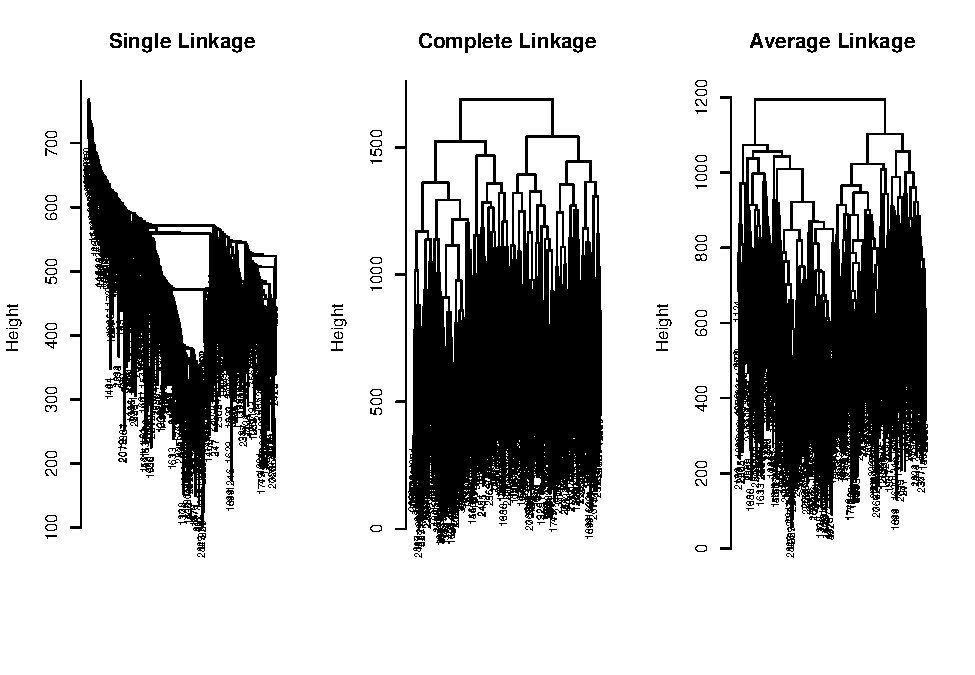
\includegraphics{Version-2_files/figure-latex/unnamed-chunk-10-1.pdf}

\begin{Shaded}
\begin{Highlighting}[]
\FunctionTok{par}\NormalTok{(}\AttributeTok{mfrow =} \FunctionTok{c}\NormalTok{(}\DecValTok{1}\NormalTok{, }\DecValTok{1}\NormalTok{))  }\CommentTok{\# Reset plot layout}
\end{Highlighting}
\end{Shaded}

Single Linkage: - The dendrogram is highly elongated with many
``chained'' clusters, where individual data points are linked
one-by-one. - This chaining effect makes it harder to distinguish clear,
well-separated clusters. - Single linkage is generally sensitive to
noise and outliers, which can result in this kind of chaining pattern.

Complete Linkage: - The dendrogram is more balanced and compact, with
clusters that appear well-separated. - This linkage method tends to
produce more spherical clusters, which is often desirable if the data
has distinct groups. - Complete linkage minimizes the maximum distance
between clusters, making it less sensitive to outliers and better suited
for identifying well-defined clusters.

Average Linkage: - The average linkage dendrogram is somewhat between
single and complete linkage in terms of cluster compactness. - Clusters
are generally balanced, though not as tight as with complete linkage.

Based on the structure observed in the dendrograms, complete linkage
seems to be the most appropriate for this dataset. It provides
well-separated, compact clusters that are less prone to the chaining
effect seen in single linkage, making it easier to interpret the
clustering structure.

\bigskip

\begin{enumerate}
\def\labelenumi{\alph{enumi}.}
\setcounter{enumi}{1}
\tightlist
\item
  {[}10 pts{]} Choose your linkage method, cut the dendrogram to obtain
  3 clusters and compare the clustering results with the true labels in
  the training dataset. What is the accuracy of the clustering? Comment
  on its performance.
\end{enumerate}

\begin{Shaded}
\begin{Highlighting}[]
\CommentTok{\# Perform complete linkage clustering on the distance matrix}
\NormalTok{hc\_complete }\OtherTok{\textless{}{-}} \FunctionTok{hclust}\NormalTok{(dist\_matrix, }\AttributeTok{method =} \StringTok{"complete"}\NormalTok{)}

\CommentTok{\# Cut the dendrogram to obtain 3 clusters}
\NormalTok{clusters }\OtherTok{\textless{}{-}} \FunctionTok{cutree}\NormalTok{(hc\_complete, }\AttributeTok{k =} \DecValTok{3}\NormalTok{)}

\CommentTok{\# Create a contingency table between true labels and predicted cluster labels}
\NormalTok{table\_result }\OtherTok{\textless{}{-}} \FunctionTok{table}\NormalTok{(true\_labels, clusters)}

\CommentTok{\# Map each cluster label to the most frequent true label within that cluster}
\NormalTok{cluster\_to\_label }\OtherTok{\textless{}{-}} \FunctionTok{sapply}\NormalTok{(}\DecValTok{1}\SpecialCharTok{:}\FunctionTok{ncol}\NormalTok{(table\_result), }\ControlFlowTok{function}\NormalTok{(col) \{}
\NormalTok{  true\_label }\OtherTok{\textless{}{-}} \FunctionTok{names}\NormalTok{(}\FunctionTok{which.max}\NormalTok{(table\_result[, col]))}
  \FunctionTok{return}\NormalTok{(true\_label)}
\NormalTok{\})}

\CommentTok{\# Convert the mapping result to a named character vector}
\FunctionTok{names}\NormalTok{(cluster\_to\_label) }\OtherTok{\textless{}{-}} \FunctionTok{colnames}\NormalTok{(table\_result)}

\CommentTok{\# Replace cluster labels with the mapped labels}
\NormalTok{mapped\_labels }\OtherTok{\textless{}{-}} \FunctionTok{as.character}\NormalTok{(cluster\_to\_label[}\FunctionTok{as.character}\NormalTok{(clusters)])}

\CommentTok{\# Calculate accuracy by comparing mapped labels to true labels}
\NormalTok{accuracy }\OtherTok{\textless{}{-}} \FunctionTok{sum}\NormalTok{(mapped\_labels }\SpecialCharTok{==}\NormalTok{ true\_labels) }\SpecialCharTok{/} \FunctionTok{length}\NormalTok{(true\_labels)}
\FunctionTok{print}\NormalTok{(}\FunctionTok{paste}\NormalTok{(}\StringTok{"Clustering Accuracy:"}\NormalTok{, }\FunctionTok{round}\NormalTok{(accuracy }\SpecialCharTok{*} \DecValTok{100}\NormalTok{, }\DecValTok{2}\NormalTok{), }\StringTok{"\%"}\NormalTok{))}
\end{Highlighting}
\end{Shaded}

\begin{verbatim}
## [1] "Clustering Accuracy: 76.2 %"
\end{verbatim}

\bigskip

\hypertarget{question-3-spectral-clustering-15-pts}{%
\section{Question 3: Spectral Clustering {[}15
pts{]}}\label{question-3-spectral-clustering-15-pts}}

For this question, let's use the spectral clustering function
\texttt{specc()} from the \texttt{kernlab} package. Let's also consider
all pixels, instead of just the top 50 features. Specify your own choice
of the kernel and the number of clusters. Report your results and
compare them with the previous clustering methods.

\begin{Shaded}
\begin{Highlighting}[]
\CommentTok{\#install.packages("kernlab")}
\FunctionTok{library}\NormalTok{(kernlab)}
\end{Highlighting}
\end{Shaded}

\begin{verbatim}
## Warning: package 'kernlab' was built under R version 4.3.3
\end{verbatim}

\begin{Shaded}
\begin{Highlighting}[]
\CommentTok{\# Specify the number of clusters (for example, using the number of unique labels in the dataset)}
\NormalTok{num\_clusters }\OtherTok{\textless{}{-}} \FunctionTok{length}\NormalTok{(}\FunctionTok{unique}\NormalTok{(mnist}\SpecialCharTok{$}\NormalTok{Digit))}

\CommentTok{\# Apply spectral clustering with an RBF kernel (Gaussian) and the specified number of clusters}
\NormalTok{spectral\_clusters }\OtherTok{\textless{}{-}} \FunctionTok{specc}\NormalTok{(}\FunctionTok{as.matrix}\NormalTok{(mnist[, }\SpecialCharTok{{-}}\DecValTok{1}\NormalTok{]), }\AttributeTok{centers =}\NormalTok{ num\_clusters, }\AttributeTok{kernel =} \StringTok{"rbfdot"}\NormalTok{)}

\CommentTok{\# Extract the cluster assignments}
\NormalTok{cluster\_labels }\OtherTok{\textless{}{-}} \FunctionTok{as.factor}\NormalTok{(spectral\_clusters}\SpecialCharTok{@}\NormalTok{.Data)}

\CommentTok{\# Compare with true labels}
\NormalTok{true\_labels }\OtherTok{\textless{}{-}}\NormalTok{ mnist}\SpecialCharTok{$}\NormalTok{Digit}
\CommentTok{\# Create a contingency table between true labels and cluster labels}
\NormalTok{table\_result }\OtherTok{\textless{}{-}} \FunctionTok{table}\NormalTok{(true\_labels, cluster\_labels)}

\CommentTok{\# Map each cluster label to the true label with the highest count in each cluster}
\NormalTok{cluster\_to\_label }\OtherTok{\textless{}{-}} \FunctionTok{apply}\NormalTok{(table\_result, }\DecValTok{2}\NormalTok{, }\ControlFlowTok{function}\NormalTok{(x) }\FunctionTok{names}\NormalTok{(}\FunctionTok{which.max}\NormalTok{(x)))}

\CommentTok{\# Replace cluster labels with mapped labels}
\NormalTok{mapped\_labels }\OtherTok{\textless{}{-}}\NormalTok{ cluster\_to\_label[}\FunctionTok{as.character}\NormalTok{(cluster\_labels)]}

\CommentTok{\# Calculate accuracy}
\NormalTok{accuracy }\OtherTok{\textless{}{-}} \FunctionTok{sum}\NormalTok{(mapped\_labels }\SpecialCharTok{==}\NormalTok{ true\_labels) }\SpecialCharTok{/} \FunctionTok{length}\NormalTok{(true\_labels)}
\FunctionTok{print}\NormalTok{(}\FunctionTok{paste}\NormalTok{(}\StringTok{"Spectral Clustering Accuracy:"}\NormalTok{, }\FunctionTok{round}\NormalTok{(accuracy }\SpecialCharTok{*} \DecValTok{100}\NormalTok{, }\DecValTok{2}\NormalTok{), }\StringTok{"\%"}\NormalTok{))}
\end{Highlighting}
\end{Shaded}

\begin{verbatim}
## [1] "Spectral Clustering Accuracy: 87.06 %"
\end{verbatim}

The accuracy is higher than all of the previous methods. \bigskip

\end{document}
